\chapter{张量网络方法介绍}
\label{chap:tensor-network}

\emph{张量网络} (tensor network)\cite{orus2014practical,bridgeman2017hand,biamonte2017tensor,orus2019tensor,ran2020tensor,evenbly2022practical}方法为凝聚态物理、量子计算\cite{markov2008simulating,huggins2019towards,yuan2021quantum}、机器学习\cite{stoudenmire2016supervised,you2018machine,liu2023tensor}\allowbreak 与可微编程\cite{liao2019differentiable,geng2022differentiable}等领域提供了一套统一的描述框架。顾名思义,张量网络就是根据一定规则连接起来张量单元,而这些局域的张量单元往往能够编码全局波函数的关键性质。相比传统的数值算法,张量网络将刻画量子态的关联与纠缠性质放在了第一优先级,因而在处理复杂的量子多体问题也具有很强的表达能力。

\section{基本概念}

张量网络中的\emph{张量} (tensor) 可以简单理解为多维数组,即标量(0 维张量)、向量(1 维张量)、矩阵(2 维张量)的推广。如图~\ref{fig:tensors} 所示,张量网络常利用图形方式来描述,其中圆圈(也可用其他图形)表示张量,延伸出来的腿表示张量的指标。

\begin{figure}[htb]
  \centering
  \tikzinput{tensor-network/basic}
  \caption[张量单元]{三种张量单元,分别对应于向量、矩阵和三阶张量。}
  \label{fig:tensors}
\end{figure}

\subsection{基本张量运算}

常用的张量运算包括张量积、缩并、变形等。

\emph{张量积} (tensor product) 相当于若干个张量并排放置,并保持指标不变:
\begin{equation}
  A_{i_1,\dots,i_r} B_{j_1,\dots,j_s} \eqcolon (A \otimes B)_{i_1,\dots,i_r,j_1,\dots,j_s}.
\end{equation}
图形描述为
\begin{equation}
  \tikzinput{tensor-network/tensor-product}
\end{equation}

张量的\emph{缩并} (contraction) 是向量内积、矩阵乘法的推广,即对两个张量的某些指标进行求和,得到一个新的张量:
\begin{equation}
  A_{abk} B_{kc} \coloneq \sum_k A_{abk} B_{kc} = C_{abc}.
\end{equation}
这里根据 Einstein 求和约定省略了求和号。张量缩并的图形描述为
\begin{equation}
  \tikzinput{tensor-network/contraction}
\end{equation}
即把需要缩并的腿(指标)连接起来。

同一个张量的指标也可以缩并。部分缩并可以得到\emph{偏迹} (partial trace),全部缩并则得到\emph{迹} (trace):
\begin{align}
     (\tr_{x,y} A)_{i_1,\dots,i_{x-1},i_{x+1},\dots,i_{y-1},i_{y+1},\dots,i_r}
  &= A_{i_1,\dots,i_{x-1},k,i_{x+1},\dots,i_{y-1},k,i_{y+1},\dots,i_r}, \\
     \tr B
  &= B_{ii}
\end{align}
其图形描述与缩并类似:
\begin{equation}
  \tikzinput{tensor-network/trace-1}
\end{equation}
利用图形语言很容易验证 $\tr(AB)=\tr(BA)$:
\begin{equation}
  \tikzinput{tensor-network/trace-2}
\end{equation}

张量的\emph{变形} (reshape) 相当于指标的重新组合,例如
\begin{equation}
  \tikzinput{tensor-network/reshape}
  \label{eq:tensor-reshape}
\end{equation}
在数值计算中,把一般形状的张量变形为矩阵,往往可以利用为矩阵优化的算法来加速计算。

\subsection{张量分解}

张量的\emph{分解} (decomposition) 可以理解为缩并的逆运算,最常用的是\emph{奇异值分解} (singular value decomposition, SVD),即
\begin{equation}
  M_{ij} = \sum_{k=1}^{\min(m,n)} U_{ik} \Lambda_{kk} V_{kj} = \sum_k U_{ik} \Lambda_{kk} \bigl( V^\dagger \bigr)_{jk},
\end{equation}
其中 $M$ 为 $m\times n$ 矩阵,$\Lambda$ 为对角矩阵(如果行数、列数不等,则相应补零),$U$ 和 $V$ 为幺正矩阵,$V^\dagger$ 表示共轭转置。利用张量的变形,可以很容易地将 SVD 推广为一般形状的张量,用图形描述为
\begin{equation}
  \tikzinput{tensor-network/svd}
\end{equation}

奇异值分解可以用来获得张量的近似表示。将奇异值($\Lambda$ 矩阵的对角元)按大小排列后,只保留前 $r$ 个值,就得到了秩为 $r$ 的近似张量:
\begin{equation}
  M_{ij} \approx \sum_{k=1}^r U_{ik} \Lambda_{kk} V_{kj}, \quad r < \min(m,n).
\end{equation}
并且可以证明,这种近似表示是所有秩为 $r$ 的张量中最优的。

对于一个一般的张量,原则上我们总可以把它改写为若干个小张量的缩并形式,并保证自由度数目不变。这种改写并不能降低计算复杂度,但我们可以利用奇异值分解把这些小张量替换为对应的近似表示,这样就可以大幅减少总自由度的数目。

在量子力学的语境中,奇异值分解也可表述为 \emph{Schmidt 分解} (Schmidt decomposition):对于 Hilbert 空间 $\mathcal{H}^{\text{L}}\otimes\mathcal{H}^{\text{R}}$,其中的任意量子态 $\ket{\Psi}$ 均可被分解为
\begin{equation}
  \ket{\Psi} = \sum_\alpha \lambda_\alpha \ket{\Phi^{\text{L}}_\alpha} \otimes \ket{\Phi^{\text{R}}_\alpha},
  \label{eq:schmidt-decomposition}
\end{equation}
其中 $\lambda_\alpha$ 称为 \emph{Schmidt 系数} (Schmidt coefficients),而 $\ket{\Phi^{\text{L}}_\alpha}$、$\ket{\Phi^{\text{R}}_\alpha}$ 分别是 $\mathcal{H}^{\text{L}}$、$\mathcal{H}^{\text{R}}$ 中的单位正交基,称为 \emph{Schmidt 向量} (Schmidt vectors)。可以发现 Schmidt 系数和奇异值是等价的,而 Schmidt 向量和幺正矩阵 $U$、$V$ 也是等价的。

\section{矩阵乘积态算法}

接下来介绍几种具体的张量网络及其算法。本文中,我们把这些算法分为两类:一类算法以矩阵乘积态为代表,主要用来处理一维量子多体系统;另一类算法则以张量重整化群为代表,顾名思义,主要用在二维网络的重整化(粗粒近似)操作中。

\subsection{波函数的构造}
\label{subsec:mps-construction}

如图~\ref{fig:mps} 所示,\emph{矩阵乘积态} (matrix product state, MPS)\cite{perez2007matrix,verstraete2008matrix,orus2014practical,cirac2021matrix}由一系列张量单元首尾相连而成,每个张量单元包含三个指标,没有缩并的称为\emph{物理指标} (physical index),另外两个则称为\emph{虚拟指标} (virtual index) 或\emph{辅助指标} (auxiliary index)。根据具体问题的需要,MPS 可取开放或周期性边界条件。当所研究的系统具有平移对称性时,可以将所有张量单元取为相同值,此时有
\begin{equation}
  % TODO: 周期性边界条件
  \Psi_{i_1 i_2 \cdots i_n} = A^{j_1 j_2}_{i_1} A^{j_2 j_3}_{i_2} \cdots A^{j_n j_1}_{i_n}.
\end{equation}
这样的张量网络称为\emph{无限 MPS} (infinite MPS, iMPS)。
% 我们之后的讨论主要针对 iMPS。

\begin{figure}[htb]
  \centering
  \subcaptionbox{开放边界条件}{\tikzinput{tensor-network/mps-1}} \qquad
  \subcaptionbox{周期性边界条件}{\tikzinput{tensor-network/mps-2}}
  \caption[矩阵乘积态]{矩阵乘积态 (MPS)。}
  \label{fig:mps}
\end{figure}

考虑一个量子态 $\ket{\Psi}$,我们对它作用一次 SVD,便可以获得由两个张量组成的 MPS,此时连接维数 $\chi$ 等于奇异值的数量。这一过程可以不断重复,以构造出任意长度的 MPS。在做 SVD 时,如果不对奇异值进行截断,可以发现 $\chi$ 会随着分解的次数(也即张量单元的数量)$N$ 指数级增长。然而对于一维\emph{有能隙} (gapped) Hamilton 量的基态以及低能激发态,$\chi$ 可以取为常数;对于\emph{无能隙} (gapless) 的临界系统,则会以多项式形式发散。

对于长度为 $L$ 的 MPS,其纠缠熵为
\begin{equation}
  S_L = -\tr(\rho_L\log\rho_L) \sim \mathcal{O}(\log\chi),
\end{equation}
其中 $\rho_L$ 是相应区块上的约化密度矩阵。这和一维有能隙 Hamilton 量基态的性质[称为\emph{面积定律} (area law)]是一致的,因此 MPS 可以较好地模拟这类系统。实际上,在全部 Hilbert 空间中,遵循面积定律的量子态仅占很少的一部分,而张量网络的结构恰好可以排除掉那些“无关”的量子态,从而大大减少了计算量。

由上述方法构造出的 MPS 并不是唯一的,而是存在所谓\emph{规范自由度} (gauge freedom)\cite{bridgeman2017hand}。如图~\ref{fig:mps-gauge-freedom} 所示,两个张量单元之间总可以插入单位矩阵 $I=XX^{-1}$,并把 $X$ 和 $X^{-1}$ 分配到两边。

\begin{figure}[htb]
  \centering
  \tikzinput{tensor-network/gauge-freedom}
  \caption[MPS 中的规范自由度]{MPS 中的规范自由度。其中张量单元 $\tilde{A}=XAX^{-1}$。}
  \label{fig:mps-gauge-freedom}
\end{figure}

% TODO: 密度矩阵
为了方便计算,我们一般会把 MPS 取为\emph{正则形式} (canonical form)\cite{orus2008infinite,schollwock2011density,orus2014practical},它要求辅助指标由 Schmidt 分解式~\eqref{eq:schmidt-decomposition} 决定。张量单元 $A$ 会被拆分成 $\Gamma$ 和 $\lambda$ 两部分,分别对应 Schmidt 向量与系数。定义左右矩阵
\begin{equation}
  \begin{aligned}
       R_{(\alpha\alpha'), \, (\beta\beta')}
    &= \sum_{i=1}^d \left( \Gamma^i_{\alpha\beta} \lambda_\beta \right) \left( \Gamma^i_{\alpha'\beta'} \lambda_{\beta'} \right)^*, \\
       L_{(\alpha\alpha'), \, (\beta\beta')}
    &= \sum_{i=1}^d \left( \lambda_\alpha \Gamma^i_{\alpha\beta} \right) \left( \lambda_{\alpha'} \Gamma^i_{\alpha'\beta'} \right)^*,
  \end{aligned}
\end{equation}
此时正则形式要求 $R$、$L$ 的特征向量均为单位矩阵(在张量变形的意义下),且对应的主特征值\footnote{即绝对值最大的特征值。它对应的特征向量也称主特征向量。} $\eta$ 相同。如图~\ref{fig:mps-canonical-form} 所示,将一般的 $\Gamma$ 和 $\lambda$(例如随机初始化的)进行正则化的方法为:

\begin{enumerate}
  \item 计算 $R$、$L$ 的主特征向量,并变形为矩阵 $V_R$、$V_L$\footnote{在实际计算中,$V_R$、$V_L$ 可能会带有冗余的相位,这会影响接下来的矩阵分解操作。此相位可通过规定 $V_R$、$V_L$ 的迹为实数来消除。},对应的特征值均为 $\eta$。将 $V_R$、$V_L$ 进一步分解为 $X$、$Y$,使其满足
    \begin{equation}
      V_R = X X^\dagger, \quad V_L = Y^\dagger Y.
    \end{equation}
    这里可以用特征值分解,也可以用 Cholesky 分解。

  \item 利用规范自由度在 $\lambda$ 两侧分别插入 $I=(Y^\trans)^{-1}Y^\trans$ 和 $I=XX^{-1}$,并对得到的 $Y^\trans\lambda X$ 进行奇异值分解:
    \begin{equation}
      Y^\trans \lambda X = U \lambda V^\dagger.
    \end{equation}

  \item 将新得到的张量重排为 $\Gamma'$
    \begin{equation}
      \Gamma' = V^\dagger X^{-1} \Gamma \left( Y^\trans \right)^{-1} U.
    \end{equation}
\end{enumerate}

可以证明通过以上步骤得到的 $\Gamma'$ 和 $\lambda'$ 的确是 iMPS 的正则形式。

\begin{figure}[htb]
  \centering
  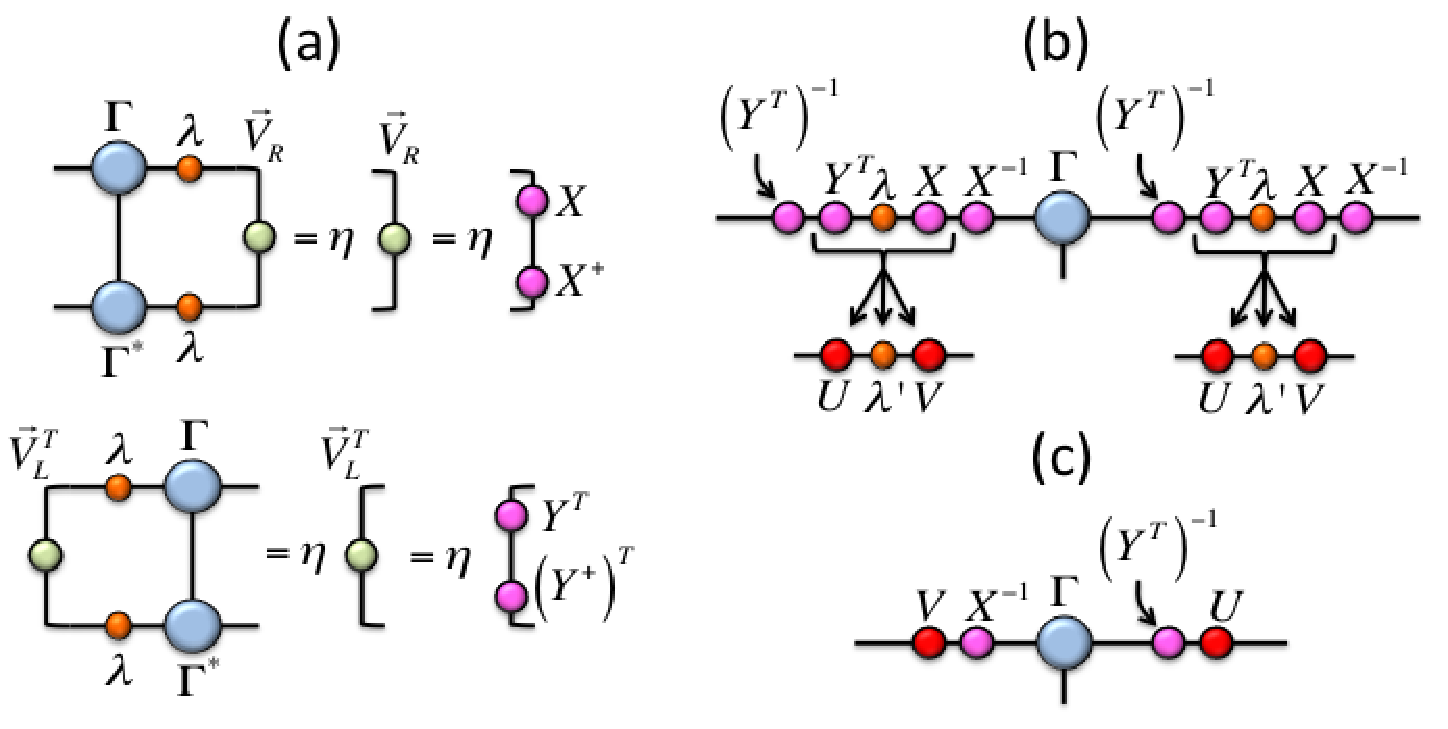
\includegraphics[width=0.85\textwidth]{images/tensor-network/mps-canonical-form.pdf}
  \caption[MPS 的正则形式]{MPS 的正则形式。(a) 计算主特征向量 $V_R$、$V_L$;(b) 利用规范自由度插入 $I=(Y^\trans)^{-1}Y^\trans$ 和 $I=XX^{-1}$,并进行 SVD;(c) 重排张量,得到 $\Gamma'$。图片来源:\parencite{orus2014practical}。}
  \label{fig:mps-canonical-form}
\end{figure}

\subsection{基态的确定}

Hamilton 量的基态 $\Psi_0$ 可以通过变分法求得:
\begin{equation}
  \ket{\Psi_0} = \argmin_{\ket{\Psi}} \frac{\langle\Psi|H|\Psi\rangle}{\langle\Psi|\Psi\rangle}.
\end{equation}
即使 $\ket{\Psi}$ 已经表示成了 MPS 的形式,一般来说也无法直接对 $\ket{\Psi}$ 进行整体优化。但是,如果 Hamilton 量能够写成图~\ref{fig:mpo} 中\emph{矩阵乘积算符} (matrix product operator, MPO) 的形式,那么就可以通过迭代算法来高效地计算 $H\ket{\Psi}$,进而通过局域优化来获得全局最优解。这实际上就是著名的\emph{密度矩阵重整化群} (density matrix renormalization group, DMRG) 算法\cite{white1992density,white1993density,schollwock2005density,mcculloch2007density,mcculloch2008infinite,schollwock2011density}。

\begin{figure}[htb]
  \centering
  \tikzinput{tensor-network/mpo}
  \caption[矩阵乘积算符]{矩阵乘积算符 (MPO)。}
  \label{fig:mpo}
\end{figure}

DMRG 的总体思路是,对正则化的 MPS 中每个张量单元 $A^{(i)}$ 依次进行优化,而这里的优化则相当于计算有效 Hamilton 量(原始 Hamilton 量 + MPS 的剩余部分)的本征态。$i$ 由 1 遍历到 $N$ 再遍历回 1 称为一次\emph{扫描} (sweep)。扫描可重复多次,直至 MPS 收敛。

根据 Lagrange 乘子法的精神,定义能量泛函为\footnote{式~\eqref{eq:dmrg-energy-functional}--\eqref{eq:dmrg-normalized-energy-equation} 中图片来源:\parencite{schollwock2011density}。}:
\begin{align}
     E[A, \tilde{A}, \lambda]
  &= \langle \Psi(A)|H|\Psi(A) \rangle - \lambda \langle \Psi(A)|\Psi(A) \rangle \notag \\
  &= \vcenter{\hbox{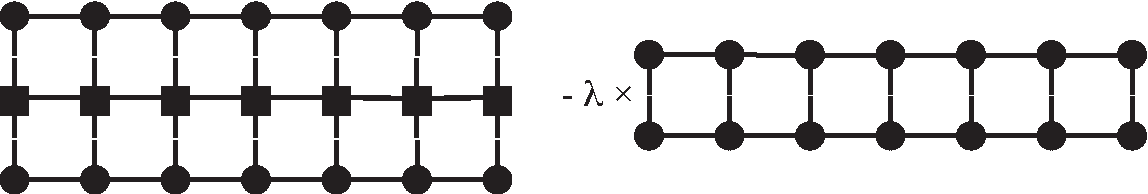
\includegraphics[height=2cm]{images/tensor-network/dmrg-energy-functional.pdf}}}.
  \label{eq:dmrg-energy-functional}
\end{align}
其中 $\lambda$ 是 Lagrange 乘子。能量取极小值的(必要)条件为
\begin{equation}
    \pdv{E[A,\tilde{A},\lambda]}{\tilde{A}^{s_i}_{\alpha_i\alpha_{i+1}}}
  = \pdv{}{\tilde{A}^{s_i}_{\alpha_i\alpha_{i+1}}} \langle \Psi(A)|H|\Psi(A) \rangle
  - \lambda \pdv{}{\tilde{A}^{s_i}_{\alpha_i\alpha_{i+1}}} \langle \Psi(A)|\Psi(A) \rangle = 0.
\end{equation}
在张量网络中,由于 $\langle\Psi(A)|H|\Psi(A)\rangle$ 和 $\langle\Psi(A)|\Psi(A)\rangle$ 都可以写成关于 $\tilde{A}^{s_i}_{\alpha_i\alpha_{i+1}}$ 的一次多项式(即其他张量与它的缩并),因此偏导数相当于在整个张量网络中“挖去” $\tilde{A}$ 的结果:
\begin{equation}
  \vcenter{\hbox{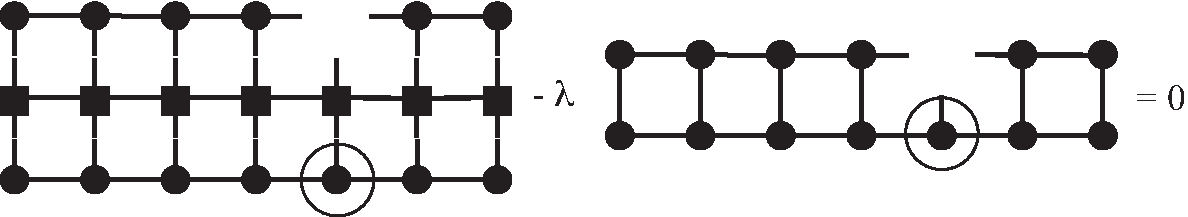
\includegraphics[height=2.2cm]{images/tensor-network/dmrg-energy-equation.pdf}}}.
\end{equation}
由于 MPS 已被正则化($R$、$L$ 的特征向量均为单位向量),上式中的第二项可以被大大简化:
\begin{equation}
  \vcenter{\hbox{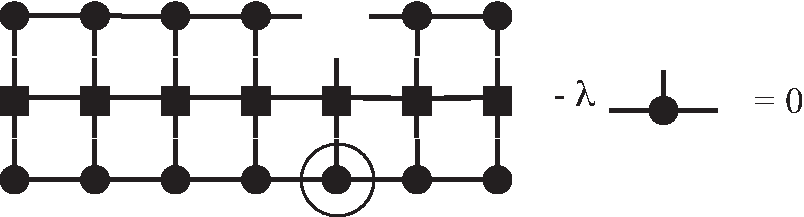
\includegraphics[height=2.2cm]{images/tensor-network/dmrg-normalized-energy-equation.pdf}}}.
  \label{eq:dmrg-normalized-energy-equation}
\end{equation}
此时,我们可以看到上式是一个关于 $A^{s'_i}_{\alpha'_i\alpha'_{i+1}}$(圆圈部分)的特征值方程:
\begin{equation}
  H_{\text{eff}} A = \lambda A,
\end{equation}
而它可以通过标准的特征值求解算法(如 Lanczos 算法)来处理。由此,我们就对 $i$ 位置处的张量单元进行了优化。

为了能够通过连接维数来控制模拟精度和计算效率,如图~\ref{fig:dmrg-two-site} 所示,我们还可以在 DMRG 中同时对两个位置的张量单元进行优化,并且利用 SVD 来得到新的 MPS。

\begin{figure}[htb]
  \centering
  \begin{tabular}{cc}
    \parbox{2em}{\subcaption{}} &
      $\vcenter{\hbox{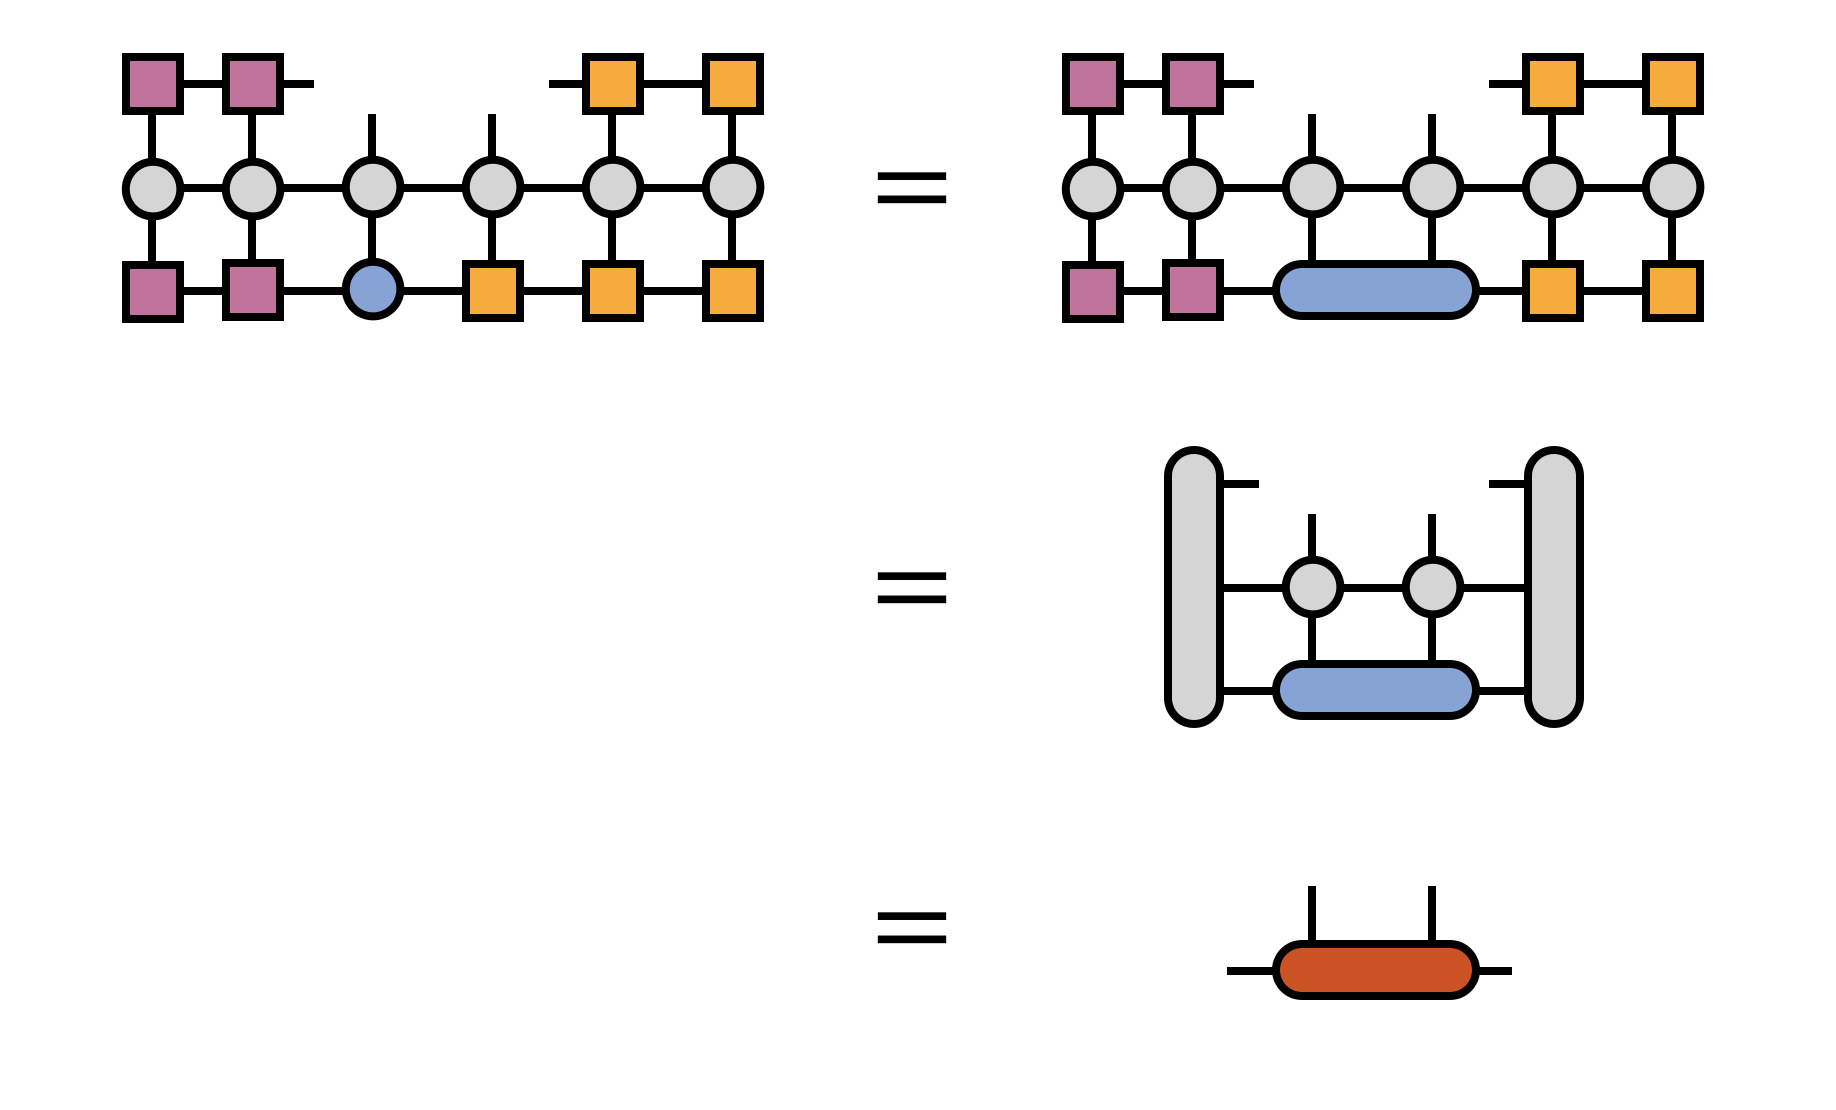
\includegraphics[width=0.7\textwidth]{images/tensor-network/dmrg-two-site.png}}}$ \\
    \parbox{2em}{\subcaption{}} &
      $\vcenter{\hbox{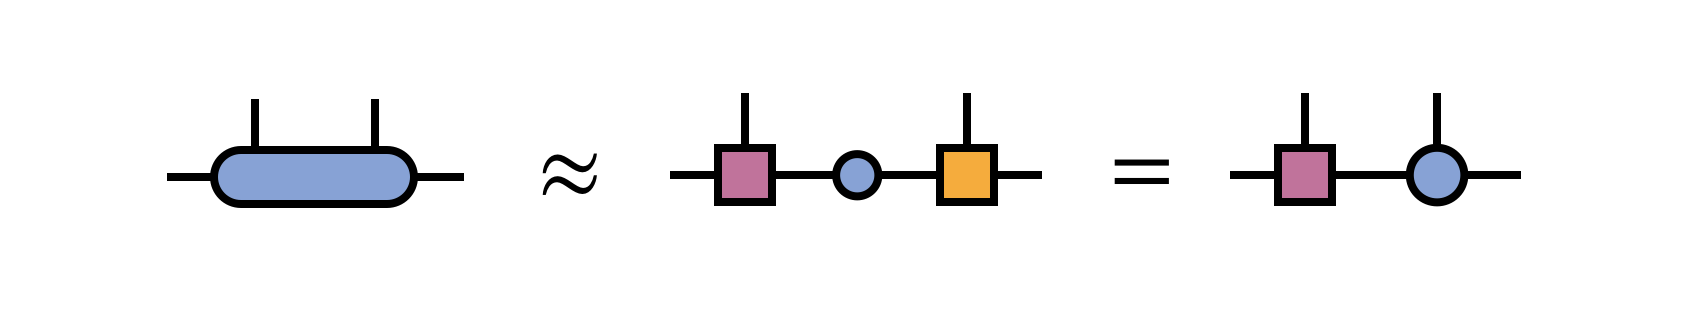
\includegraphics[width=0.7\textwidth]{images/tensor-network/dmrg-two-site-svd.png}}}$
  \end{tabular}
  \caption[两位置上 DMRG 算法]{两位置上 DMRG 算法。(a) 两个 MPS 张量单元首先缩并,再和 $H$ 缩并,得到 $H_{\text{eff}}$。(b) 利用 SVD 来得到新的 MPS。图片来源:\url{https://tensornetwork.org/mps/algorithms/dmrg/}。}
  \label{fig:dmrg-two-site}
\end{figure}

\subsection{时间演化}
\label{subsec:mps-time-evolution}

下面我们介绍\emph{无限时间演化块消减} (infinite time-evolving block decimation, iTEBD)\cite{vidal2007classical,orus2008infinite}算法,它主要用来处理波函数的时间演化
\begin{equation}
  \ket{\Psi_t} = \ee^{-\ii Ht} \ket{\Psi_0}
\end{equation}
或虚时演化
\begin{equation}
  \ket{\Psi_\tau} = \ee^{-H\tau} \ket{\Psi_0},
\end{equation}
其核心在于通过 Suzuki--Trotter 分解\cite{sornborger1999higher}
\begin{equation}
  \ee^{-\tau(A+B)} = \ee^{-\tau A} \ee^{-\tau B} + \mathcal{O}(\tau^2)
\end{equation}
将演化算符表示成 MPO 的形式,这样就可以很方便地与 MPS 形式的波函数进行缩并。

对于时间演化或虚时演化算符而言,由于经过 Suzuki--Trotter 分解后它们都很接近幺正算符,不会破坏 iMPS 的正则形式。而一般的算符并不具备这一性质,所以需要额外进行正则化操作。如图~\ref{fig:itebd-evolution} 所示,一般的 iTEBD 算法如下:

\begin{enumerate}
  \item 取随机的 iMPS $\{\Gamma,\lambda\}$,并按照 \ref{subsec:mps-construction} 小节中介绍的方法将其正则化。

  \item 把 $\{\Gamma,\lambda\}$ 与 MPO 的张量单元进行缩并:
    \begin{equation}
      \tilde{\Gamma}_{j\tilde{\alpha}\tilde{\beta}} = \sum_{i=1}^d \Gamma_{i\alpha\beta} O_{ij\mu\nu}, \quad
      \tilde{\lambda}_{\tilde{\beta}} = \lambda_\beta.
    \end{equation}
    这里指标 $\tilde{\alpha}=(\alpha,\mu)$、$\tilde{\beta}=(\beta,\nu)$,因此得到的 iMPS 对应连接维数 $\tilde{\chi}=\kappa\chi$。

  \item 对 $\{\tilde{\Gamma},\tilde{\lambda}\}$ 进行正则化,得到 $\{\tilde{\Gamma}',\tilde{\lambda}'\}$。

  \item 利用奇异值分解对 $\{\tilde{\Gamma}',\tilde{\lambda}'\}$ 进行截断,即只保留前 $\chi$ 个奇异值,使得连接维数保持在 $\chi$。

  \item 重复步骤 2--4,直到 iMPS 收敛。
\end{enumerate}

\begin{figure}[htb]
  \centering
  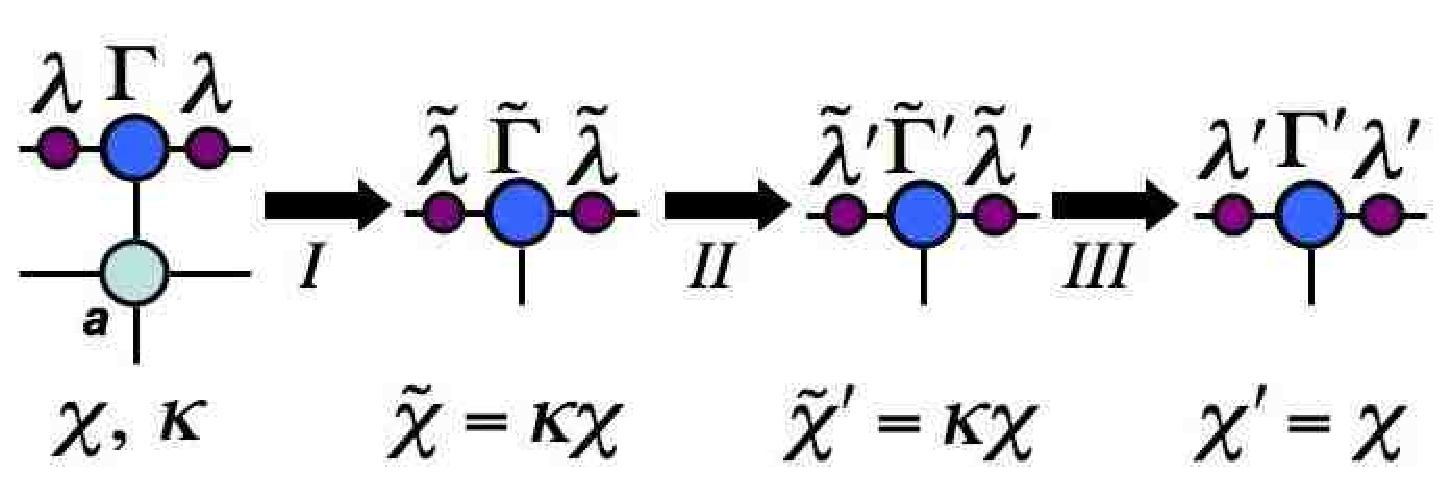
\includegraphics[width=0.6\textwidth]{images/tensor-network/itebd-evolution.pdf}
  \caption[iTEBD 算法]{iTEBD 算法。(I) 把 iMPS $\{\Gamma,\lambda\}$ 与 MPO 的张量单元进行缩并;(II) 对 $\{\tilde{\Gamma},\tilde{\lambda}\}$ 进行正则化;(III) 利用 SVD 把连接维数保持在 $\chi$。图片来源:\parencite{orus2008infinite}。}
  \label{fig:itebd-evolution}
\end{figure}

\subsection{配分函数的计算}
\label{subsec:partition-function}

一个不同于时间(虚时)演化的例子,是把二维经典格点模型的配分函数视为 iMPS 在转移矩阵作用下的演化:
\begin{equation}
  Z(\beta) = \lim_{p,q\to\infty} \omega^{pq},
\end{equation}
其中 $\omega$ 是 $W$ 矩阵的主特征值\cite{orus2008infinite}:
\begin{equation}
  \vcenter{\hbox{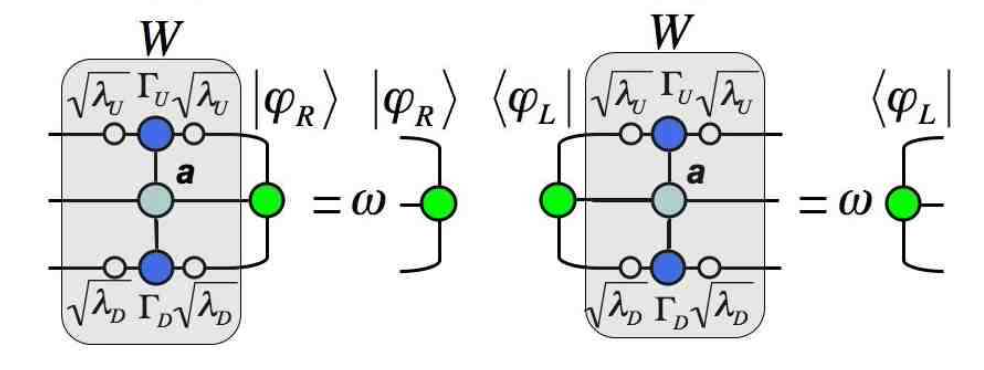
\includegraphics[width=0.7\textwidth]{images/tensor-network/itebd-w-matrices.png}}}
\end{equation}
此时我们还可以计算单点函数和两点(关联)函数的期望值:
\begin{equation}
  \begin{aligned}
    \ev[\big]{f(\sigma^{\bm{r}})}
      &= \frac{1}{Z(\beta)} \sum_{\{\sigma\}} f(\sigma^{\bm{r}}) \, \ee^{-\beta H(\{\sigma\})}, \\
    \ev[\big]{f(\sigma^{\bm{r}}) g(\sigma^{\bm{r}'})}
      &= \frac{1}{Z(\beta)} \sum_{\{\sigma\}} f(\sigma^{\bm{r}}) g(\sigma^{\bm{r}'}) \, \ee^{-\beta H(\{\sigma\})}.
  \end{aligned}
\end{equation}
主要思路是将原配分函数中的张量单元 $A$ 替换为包含 $f(s)$ 或 $g(s)$ 的 $B$ 或 $B'$,并用同样的方法进行缩并。如图~\ref{fig:expectation-value} 所示,由于 iMPS 已被正则化,我们只需处理一个较小的张量网络。

\begin{figure}[htb]
  \centering
  \subcaptionbox{}{%
    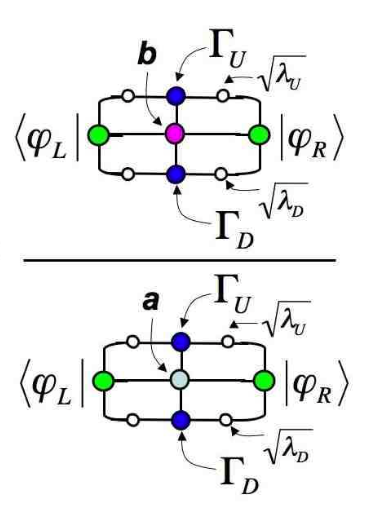
\includegraphics[height=6.5cm]{images/tensor-network/itebd-one-point-function.png}} \quad
  \subcaptionbox{}{%
    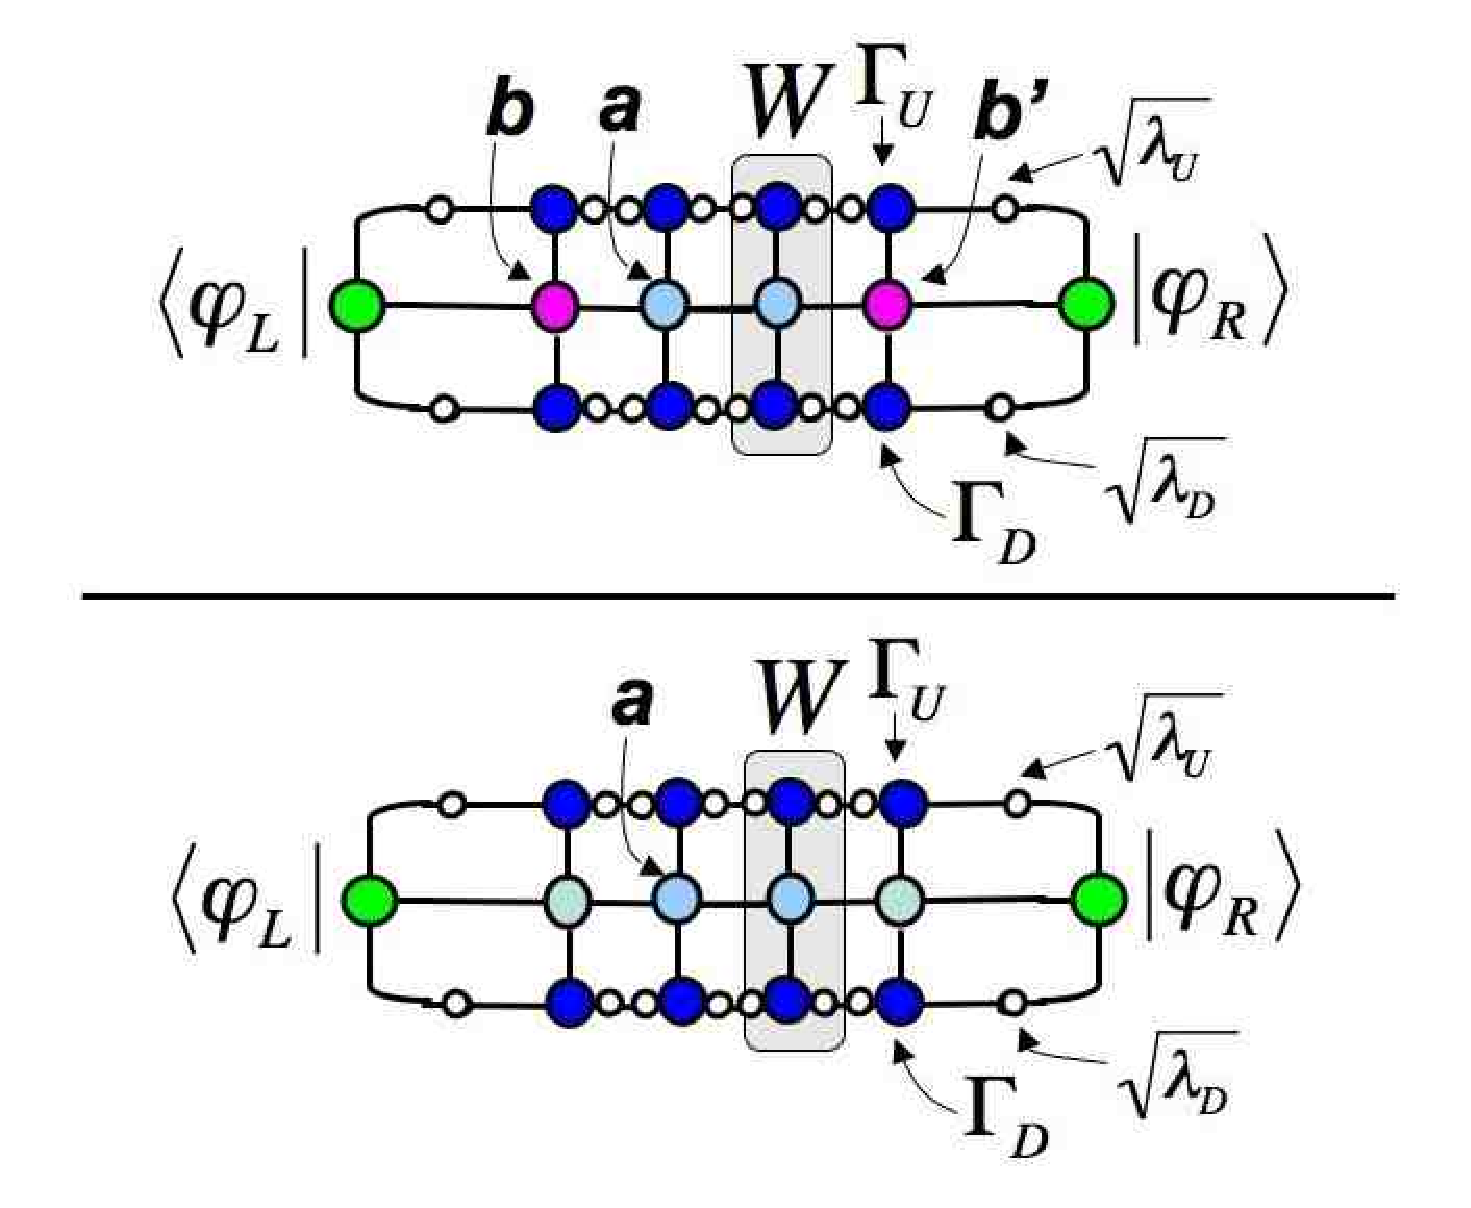
\includegraphics[height=6.5cm]{images/tensor-network/itebd-two-point-function.pdf}}
  \caption[单点函数和两点关联函数的计算]{(a) 单点函数和 (b) 两点(关联)函数的计算。图片来源:\parencite{orus2008infinite}。}
  \label{fig:expectation-value}
\end{figure}

\subsection{推广}
\label{subsec:mps-generalization}

如图~\ref{fig:peps} 所示,MPS 向高维的自然推广就得到了\emph{投影纠缠对态} (projected entangled pair state, PEPS)\cite{verstraete2004renormalization,orus2014practical,cirac2021matrix} 张量网络。对于长宽均为 $L$、连接维数为 $\chi$ 的 PEPS,其纠缠熵满足
\begin{equation}
  S_L \sim \mathcal{O}(L\log\chi),
\end{equation}
这与二维系统的面积定律也是相一致的。此外,PEPS 可以准确描述幂律形式的关联函数,因此可以用来处理一维的量子临界系统(可通过经典—量子模型的映射来实现)。但与一维的 MPS 不同,在 PEPS 中无法为所有指标同时指定一组正交基,因此并不能精确定义正则形式。

\begin{figure}[htb]
  \centering
  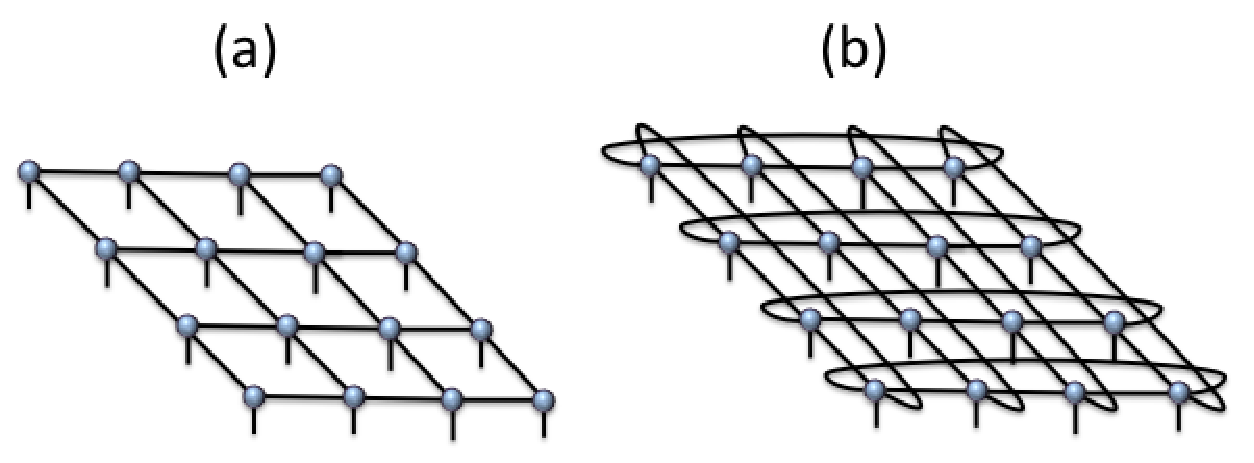
\includegraphics[width=0.8\textwidth]{images/tensor-network/peps.pdf}
  \caption[投影纠缠对态]{投影纠缠对态。图 (a)、(b) 分别对应开放和周期性边界条件。图片来源:\parencite{orus2014practical}。}
  \label{fig:peps}
\end{figure}

另一种用来近似表示一维系统的张量网络是\emph{多尺度纠缠重整化方法} (multiscale entanglement renormalization ansatz, MERA)\cite{vidal2007entanglement,evenbly2009algorithms,konig2009exact,evenbly2014algorithms,evenbly2015tensor2}。如图~\ref{fig:mera} 所示,MERA 使用了一组幺正变换
\begin{equation}
  u \colon \mathbb{V} \otimes \mathbb{V} \to \mathbb{V} \otimes \mathbb{V}, \quad
  u u^\dagger = I^{\otimes2}
\end{equation}
和投影算符
\begin{equation}
  v \colon \mathbb{V} \to \mathbb{V} \otimes \mathbb{V}, \quad
  v^\dagger v = I
\end{equation}
来构建粗粒近似的波函数,其中 $\mathbb{V}=\mathbb{C}^\chi$ 是 $\chi$ 维复向量空间。这里的 $u$ 和 $v$ 分别称为\emph{解纠缠子} (disentangler) 和\emph{等距子} (isometry)。解纠缠子可以消除短程纠缠的影响,因而其纠缠熵满足
\begin{equation}
  S_L \sim \mathcal{O}(\log L).
\end{equation}
这就使得 MERA 张量网络可以较好地近似一维无能隙的临界系统。

\begin{figure}[htb]
  \centering
  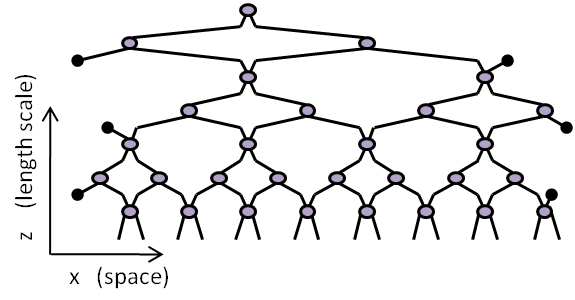
\includegraphics[width=0.6\textwidth]{images/tensor-network/mera.pdf}
  \caption[多尺度纠缠重整化方法]{多尺度纠缠重整化方法。其中两条腿进、两条腿出的张量单元是解纠缠子 $u$,而两条腿进、一条腿出的张量单元则是等距子 $v$。图片来源:\parencite{evenbly2011tensor}。}
  \label{fig:mera}
\end{figure}

\section{重整化算法}
\label{sec:tensor-network-rg}

接下来我们主要考察二维张量网络。与 \ref{subsec:partition-function} 小节相同,我们关注的一个核心问题仍然是格点模型配分函数的计算。类似于 Kadanoff 的实空间重整化群\cite{pathria2011statistical},张量重整化算法的主要思路是对张量网络进行粗粒近似,直到得到一个不动点张量。

\subsection{张量重整化群}

最基本的一种重整化算法称为\emph{张量重整化群} (tensor renormalization group, TRG)\cite{levin2007tensor}。其步骤为\footnote{式~\eqref{eq:trg-factorizing-svd}--\eqref{eq:trg-partition-function} 中图片来源:\url{https://tensornetwork.org/trg/}。}:

\begin{enumerate}
  \item 利用 SVD 对原始的张量单元 $A^{(0)}$ 进行分解:
    \begin{align}
      & \vcenter{\hbox{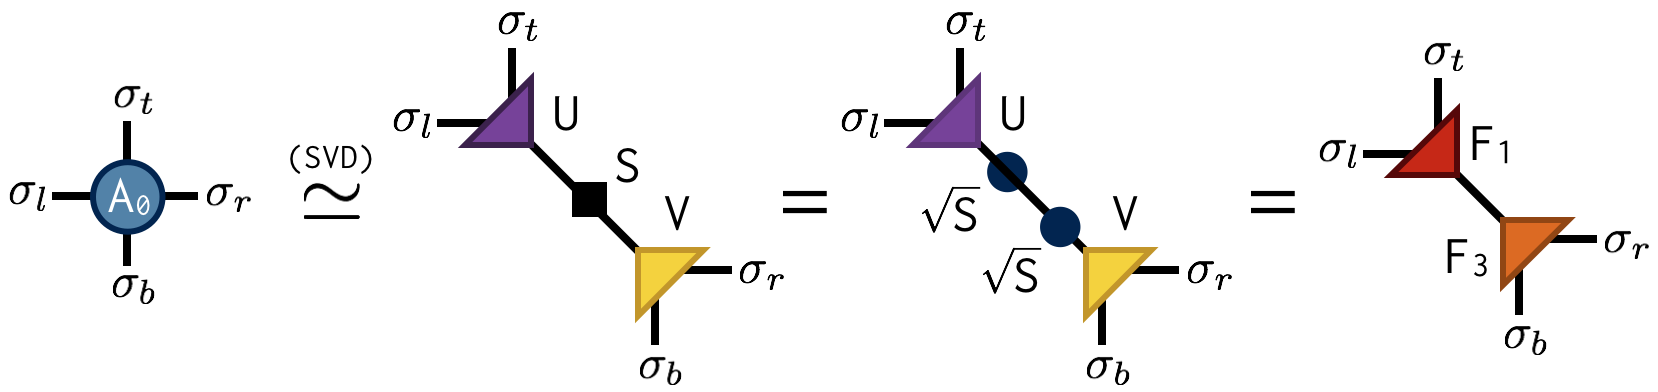
\includegraphics[width=0.8\linewidth]{images/tensor-network/trg-factorizing-svd.png}}}
        \label{eq:trg-factorizing-svd} \\
      & \vcenter{\hbox{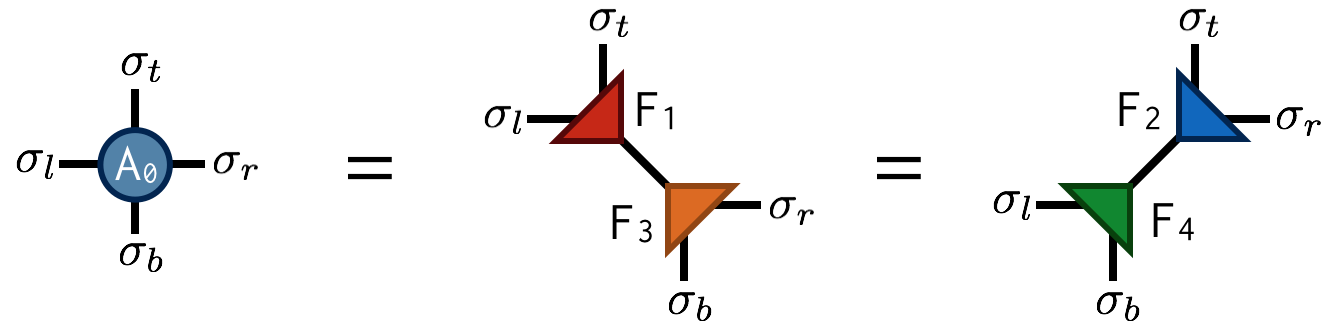
\includegraphics[width=0.65\linewidth]{images/tensor-network/trg-factorizing.png}}}
    \end{align}
    在做 SVD 时需要对奇异值进行截断,即只保留 $\chi$ 个最大奇异值,这样可以保证 TRG 的计算开销始终在可控范围内。

  \item 把得到的三角形张量缩并为新的张量单元 $A^{(1)}$:
    \begin{equation}
      \vcenter{\hbox{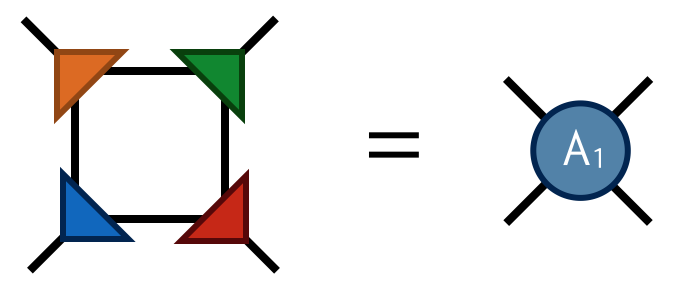
\includegraphics[width=0.35\linewidth]{images/tensor-network/trg-group.png}}}
    \end{equation}
    此时的张量网络相当于旋转了 $45^\circ$,而总的张量数目减少了一半。

  \item 重复以上步骤,直至收敛到不动点张量。

  \item 对最终得到的不动点张量进行求迹操作即可得到配分函数 $Z$:
    \begin{equation}
      Z = \sum_{i,j} A^{(N)}_{ijij}
        = \vcenter{\hbox{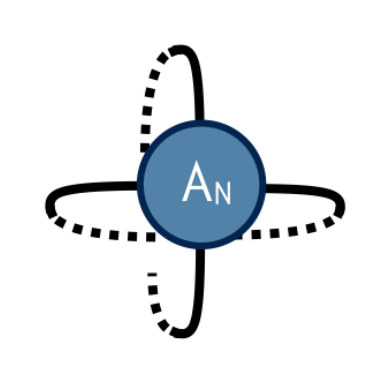
\includegraphics[width=2cm]{images/tensor-network/trg-double-trace.png}}}
      \label{eq:trg-partition-function}
    \end{equation}
\end{enumerate}

在实际计算中直接对 $A^{(n)}$ 进行缩并会很快使数值溢出。一种常用的技术是在每一步中对 $A^{(n)}$ 进行归一化,即令其 Frobenius 范数
\begin{equation}
  \bigl| A^{(n)} \bigr|_{\mathrm{F}} = \left( \sum_{i,j,k,l} A^{(n)}_{ijkl} \right)^{1/2} = 1,
\end{equation}
并记录每步所得的范数。最终的配分函数就相当于不动点张量 $A^{(N)}$ 与这些范数的乘积。如图~\ref{fig:trg-ising} 所示,我们利用 TRG 算法计算了二维 Ising 模型的配分函数、能量及热容。这一方法实现简单、计算快捷,但可以看到在临界点处其结果与精确值仍有一定差异。

\begin{figure}[htb]
  \centering
  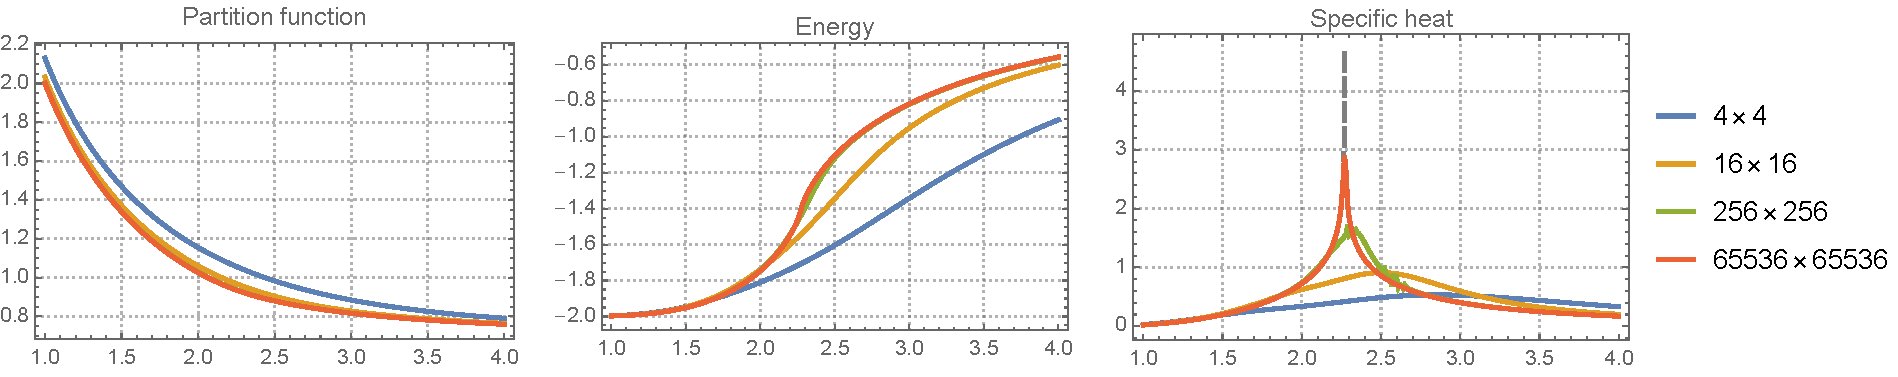
\includegraphics[width=\textwidth]{images/tensor-network/trg-ising.pdf}
  \caption[利用 TRG 算法计算得到的二维 Ising 模型的各物理量]{利用 TRG 算法计算得到的二维 Ising 模型的配分函数、能量及热容。横坐标为温度,纵坐标为各物理量在单位格点上的取值,不同颜色的曲线代表不同的系统尺寸($2^N\times2^N$,其中 $N$ 为 TRG 步数)。计算中选取连接维数 $\chi=16$。可以发现在临界点处 TRG 的计算结果与精确值(用虚线标记)仍有一定差异。}
  \label{fig:trg-ising}
\end{figure}

\subsection{张量网络重整化}

TRG 算法对于临界的格点模型效果并不好。这主要是由于临界系统中存在长程关联,纠缠熵
\begin{equation}
  S = -\tr(\rho\log\rho)
\end{equation}
会随着系统尺寸以对数级增长,然而通过 SVD 给出的张量分解并不能很好地保留这些信息。

如图~\ref{fig:tnr} 所示,TRG 的一种改进算法称为\emph{张量网络重整化} (tensor network renormalization, TNR)\cite{evenbly2015tensor1,evenbly2017algorithms},它借鉴了 MERA 的思想,同样使用解纠缠子 (disentangler) 和等距子 (isometry) 张量单元来实现粗粒近似。它们的具体取值可以通过最小化截断误差\cite{evenbly2015tensor1}
\begin{equation}
  \delta = \vcenter{\hbox{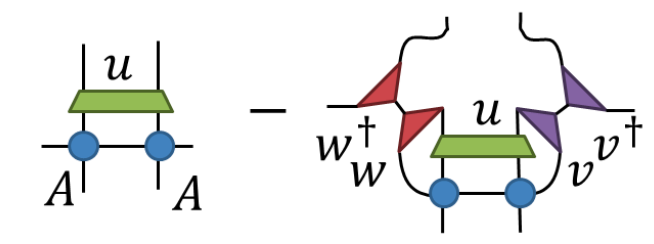
\includegraphics[width=6cm]{images/tensor-network/tnr-truncation-error.png}}}
\end{equation}
来获得。利用角双线 (corner double line, CDL) 张量的方法可以证明\cite{evenbly2015tensor1,hauru2018renormalization},TNR 算法中的 $u$ 和 $v$ 可以消除短程纠缠的影响,使得最终获得的不动点张量的确是标度不变的。

\begin{figure}[htb]
  \centering
  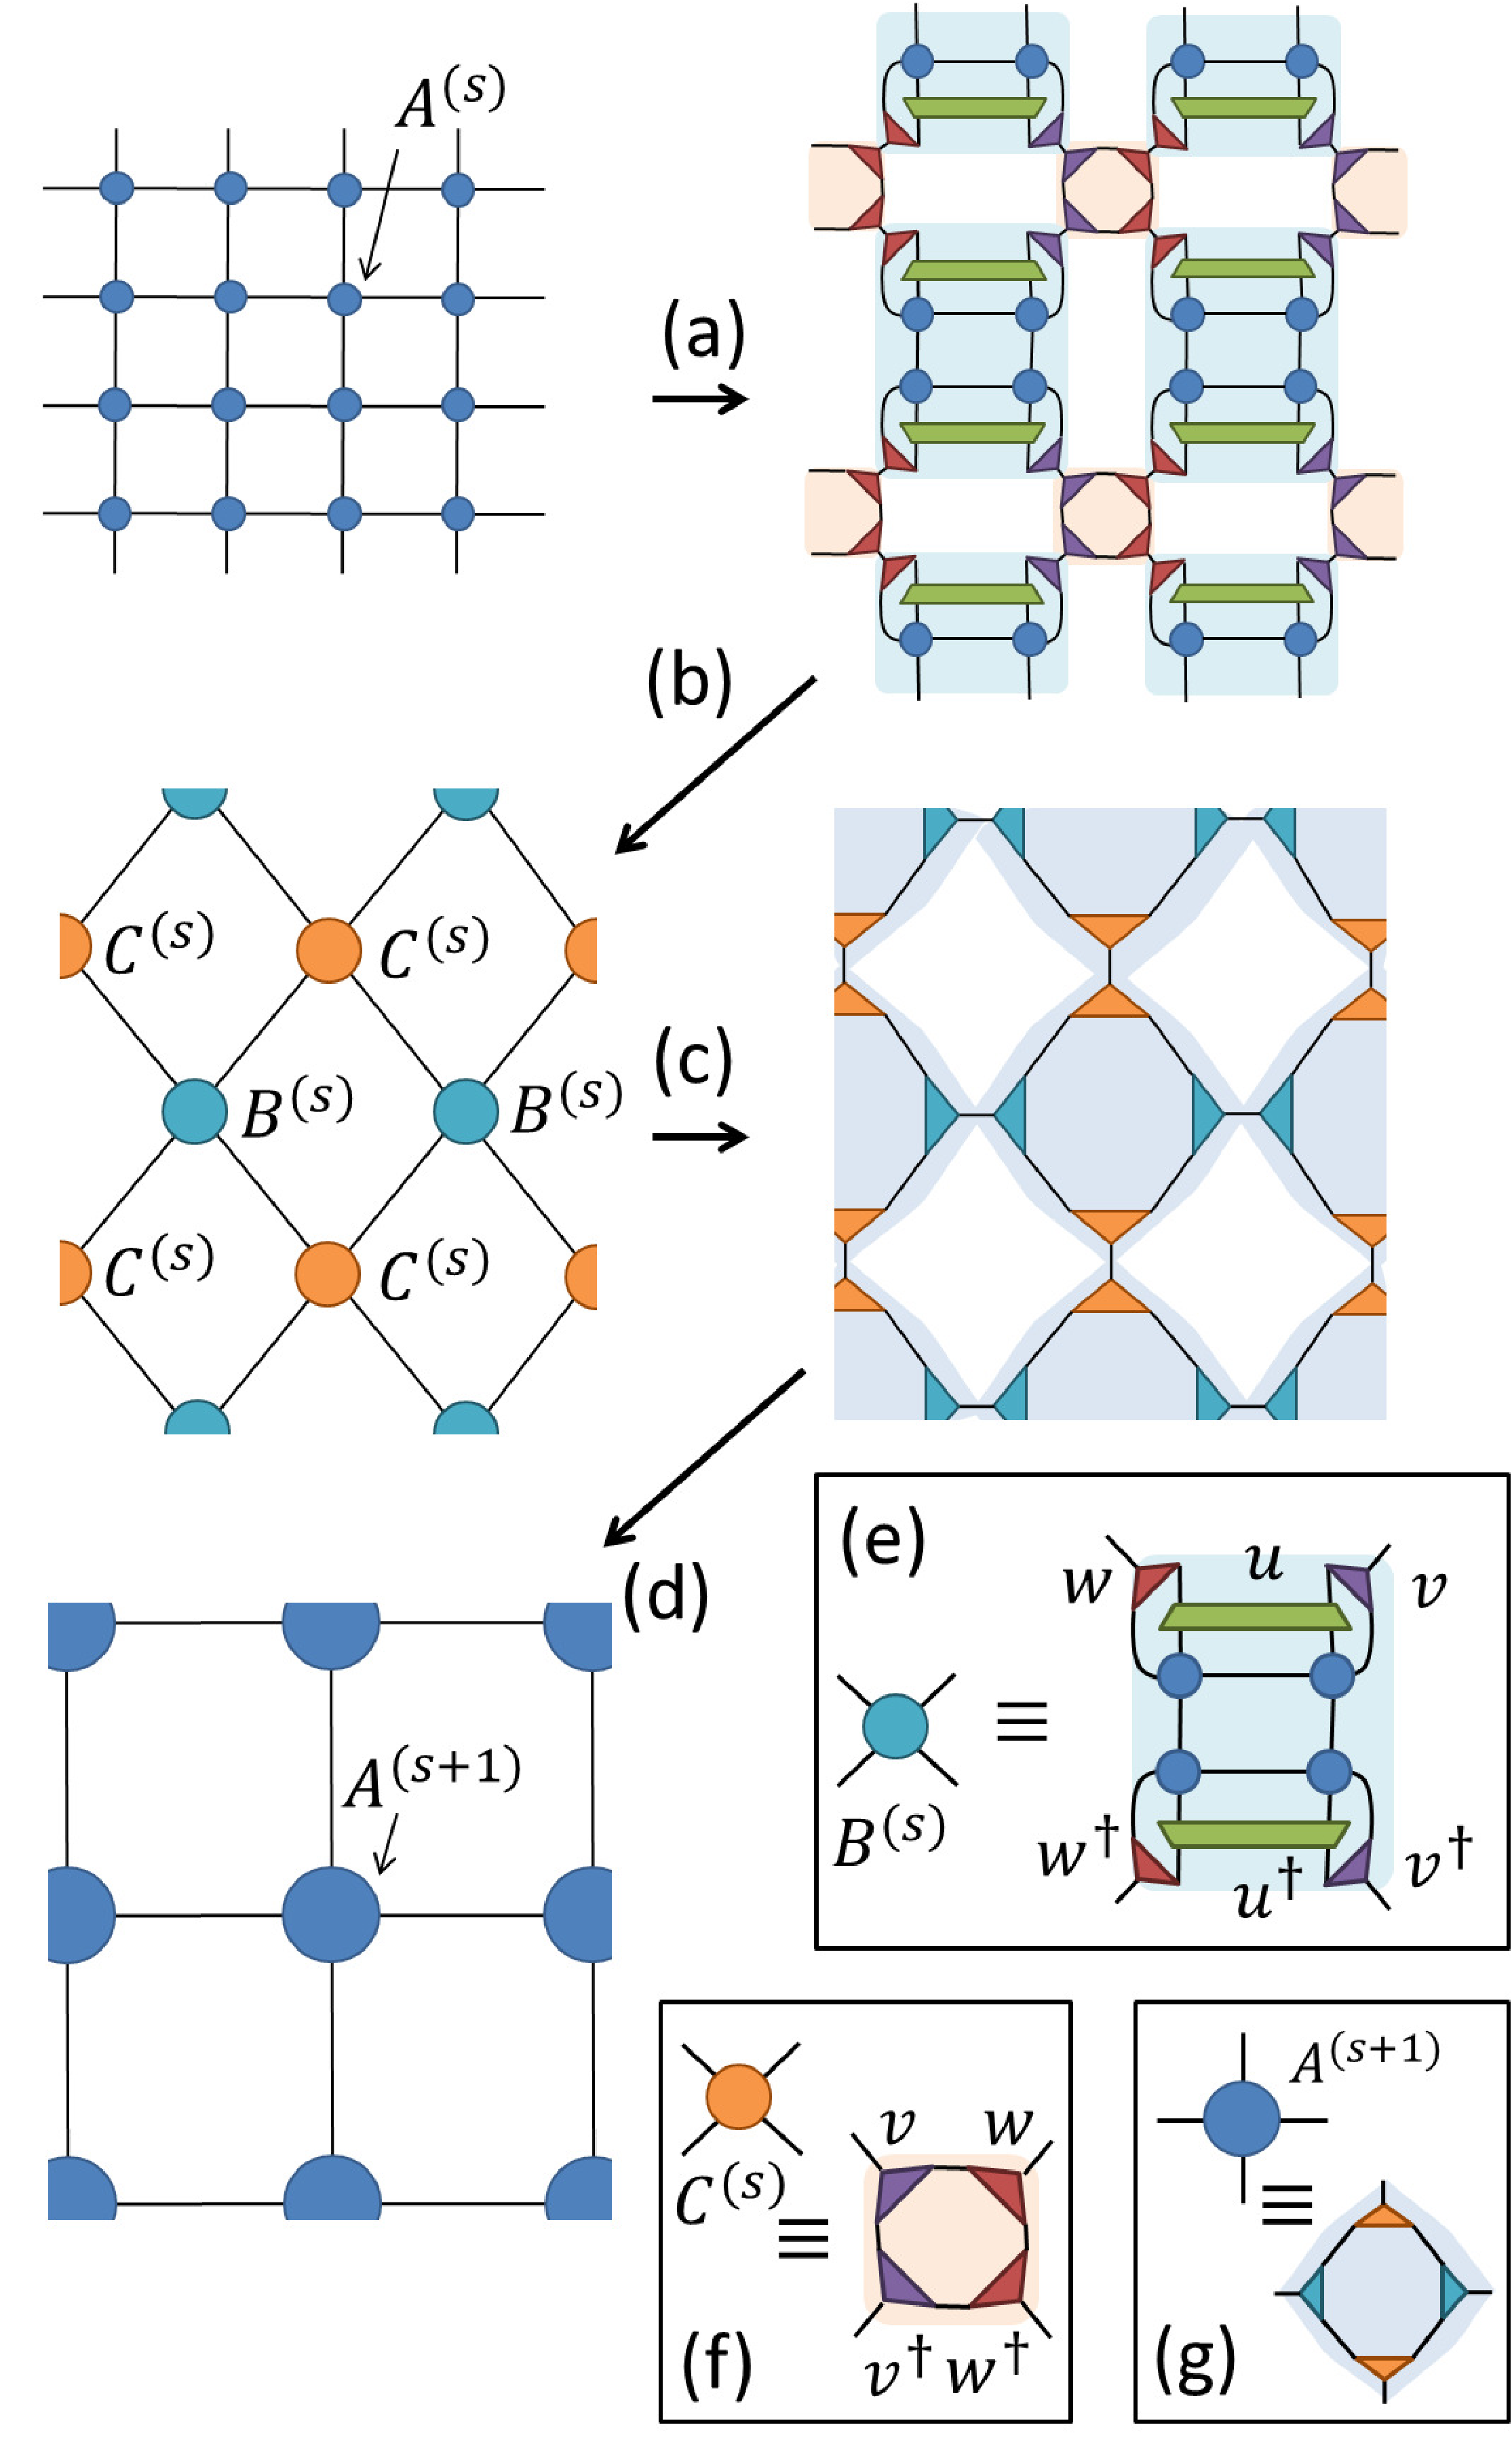
\includegraphics[width=0.6\textwidth]{images/tensor-network/tnr.pdf}
  \caption[TNR 算法]{TNR 算法。(a) 在 $2\times2$ 个 $A^{(s)}$ 张量单元之间插入解纠缠子 $u$ 和等距子 $v$。(b) 缩并得到辅助张量 $B^{(s)}$ 和 $C^{(s)}$。(c) 与 TRG 类似,利用 SVD 分解张量 $B^{(s)}$ 和 $C^{(s)}$。(d) 缩并得到新的张量单元 $A^{(s+1)}$。(e)--(g) 张量 $B^{(s)}$、$C^{(s)}$ 和 $A^{(s+1)}$ 的具体定义。图片来源:\parencite{evenbly2015tensor1}。}
  \label{fig:tnr}
\end{figure}

除了 TNR 之外,还有其他一些工作试图改进原始的 TRG 算法,如利用张量乘积态作为试探波函数的\emph{张量纠缠重整化群} (tensor-entanglement renormalization group, TERG) 算法\cite{gu2008tensor}、引入过滤操作以消除短程纠缠影响的\emph{张量纠缠过滤重整化} (tensor entanglement-filtering renormalization, TEFR) 算法\cite{gu2009tensor1}、基于高阶奇异值分解的\emph{高阶 TRG} (higher order TRG, HOTRG) 算法\cite{xie2012coarse}以及通过将小张量组合成环路并加以优化的\emph{环路 TNR} (loop TNR) 算法\cite{yang2017loop}等。这些方法相比 TRG 和 TNR 在精度、计算效率与适用范围上各有优劣,需要根据具体问题加以权衡。

\section{具体实现}

本文后续介绍的算法主要使用 Python 语言实现,其中的张量运算则利用 NumPy\cite{harris2020array}、SciPy\cite{virtanen2020scipy}编写。它们提供了高效的张量缩并、变形以及 SVD、特征值求解等算法,并且还能通过线性算符 (linear operator) 的方法处理较大规模的稀疏矩阵与张量。此外,在硬件支持的情况下,还可以借助 GPU 甚至 TPU\cite{ganahl2023density}进一步加速计算过程。

近年来,人们使用多种语言编写了各类张量网络程序包,例如基于 MATLAB 的 NCON\cite{pfeifer2014ncon},基于 Python 的 TeNPy\cite{hauschild2018efficient}、TensorNetwork\cite{roberts2019tensornetwork}以及基于 Julia 的 TensorOperations.jl\cite{jutho2023tensoroperations}等。特别值得注意的是基于 C++ 和 Julia 实现的 ITensor\cite{fishman2022itensor}包,它能够根据指标本身的性质自动完成张量缩并,无需手动选择求和指标。文献 \parencite{psarras2021landscape} 对这些程序包的功能和特点进行了总结和比较。

在处理较大的系统时,张量缩并往往会成为计算瓶颈。为此人们提出了一系列优化方案\cite{pfeifer2014faster,evenbly2014improving},以寻找最优的缩并路径。NCON、opt\_einsum\cite{daniel2018opteinsum}等程序包中均给出了实现。

\section{本章小结}

本章主要通过图形方式介绍了张量网络方法,其中重要的运算包括张量缩并和基于 SVD 的张量分解等。我们着重讨论了一维和二维下两类张量网络算法,分别以矩阵乘积态 (MPS) 和张量重整化群 (TRG) 为代表。对于 MPS 而言,密度矩阵重整化群 (DMRG) 算法可以用来获得基态,而无限时间演化块消减 (iTEBD) 算法则可以用来处理波函数的时间演化。TRG 主要用来计算二维格点系统的配分函数,其推广张量网络重整化 (TNR) 算法可以消除短程纠缠的影响,从而能够更准确地模拟临界系统。最后,我们还简要介绍了一些常用的张量网络程序包。
